%%%%%%%%%%%%%%%%%%%%%%%%%%%%%%%%%%%%%%%%%
% Professional Mathematical Presentation Template
% 
% This template uses the beamer class with the Madrid theme
% and a custom color scheme for a clean, professional look
% that works well with mathematical content.
%%%%%%%%%%%%%%%%%%%%%%%%%%%%%%%%%%%%%%%%%

\documentclass[aspectratio=169]{beamer} % 16:9 aspect ratio (modern)

% Theme settings
\usetheme{Madrid}
\usecolortheme{default}


\definecolor{primcolor}{RGB}{25,50,100} % Dark blue
\setbeamercolor{structure}{fg=primcolor}
\setbeamercolor{frametitle}{bg=primcolor!15, fg=primcolor}
\setbeamercolor{title}{fg=white} % White title text for contrast
\setbeamercolor{subtitle}{fg=white} % White subtitle text
\setbeamercolor{author}{fg=primcolor} % White author text
\setbeamercolor{date}{fg=primcolor} % White date text
\setbeamercolor{institute}{fg=primcolor} % White institute text

% Font settings
\usefonttheme{professionalfonts}
\usefonttheme{serif}

% Package imports
\usepackage{amsmath, amsfonts, amssymb, amsthm} % Math packages
\usepackage{mathtools} % Enhanced math tools
\usepackage{bm} % Bold math symbols
\usepackage{graphicx} % For images
\usepackage{booktabs} % Professional tables
\usepackage{tikz} % For diagrams
\usetikzlibrary{arrows, positioning, matrix, decorations.pathreplacing}

% Use beamer's theorem styles
\setbeamertemplate{theorem}[ams style]
\setbeamertemplate{theorems}[numbered]


% Remove navigation symbols
\setbeamertemplate{navigation symbols}{}

% Custom footer
\setbeamertemplate{footline}{
  \leavevmode%
  \hbox{%
  \begin{beamercolorbox}[wd=.333333\paperwidth,ht=2.25ex,dp=1ex,center]{author in head/foot}%
    \usebeamerfont{author in head/foot}\insertshortauthor
  \end{beamercolorbox}%
  \begin{beamercolorbox}[wd=.333333\paperwidth,ht=2.25ex,dp=1ex,center]{title in head/foot}%
    \usebeamerfont{title in head/foot}\insertshorttitle
  \end{beamercolorbox}%
  \begin{beamercolorbox}[wd=.333333\paperwidth,ht=2.25ex,dp=1ex,right]{date in head/foot}%
    \usebeamerfont{date in head/foot}\insertshortdate{}\hspace*{2em}
    \insertframenumber{} / \inserttotalframenumber\hspace*{2ex} 
  \end{beamercolorbox}}%
  \vskip0pt%
}

% Title information
\title[DP2]{Dynamic Programming}
\subtitle{Thomas J. Sargent and John Stachurski}
\author[Longye]{Longye Tian \\ \texttt{longye.tian@anu.edu.au}}
\institute[ANU]{Australian National University\\ School of Economics}
\date{March 7th, 2025}
\DeclareFontFamily{U}{mathx}{\hyphenchar\font45}
\DeclareFontShape{U}{mathx}{m}{n}{
      <5> <6> <7> <8> <9> <10>
      <10.95> <12> <14.4> <17.28> <20.74> <24.88>
      mathx10
      }{}
\DeclareSymbolFont{mathx}{U}{mathx}{m}{n}
\DeclareMathSymbol{\bigtimes}{1}{mathx}{"91}

\begin{document}

% Title frame
\begin{frame}
  \titlepage
\end{frame}

% Outline frame
\begin{frame}{Outline}
  \tableofcontents
\end{frame}

% Section 1
\section{Section 1.2.1 Definitions and Properties}
\subsection{1.2.1.1-1.2.1.3 Definition and Bellman operator}
\begin{frame}{Definitions}
    \begin{definition}
        We define an \textbf{abstract dynamic program (ADP)} to be a pair $V,\mathbb{T}$, where
        \begin{enumerate}
            \item[(i)] $V = (V,\precsim)$ is a partially ordered set
            \item[(ii)] $\mathbb{T} = \{T_\sigma: \sigma\in\Sigma\}$ is a nonempty family of order preserving self-maps on $V$.
        \end{enumerate}
    \end{definition}
    \begin{definition}
        \begin{itemize}
            \item $V$ is called the \textbf{value space}
            \item Each operator $T_\sigma\in\mathbb{T}$ is called the \textbf{policy operator}
            \item $\Sigma$ is an arbitrary index set and elements of $\Sigma$ is called \textbf{policy}
            \item We denote the unique fixed point of $T_\sigma$ as $v_\sigma$ and call it the $\sigma$-value function.
            \item We say that $\sigma\in\Sigma$ is \textbf{$v$-greedy} if $T_\tau v\precsim T_\sigma v$ for all $\sigma\in\Sigma$, i.e., $\sigma$ is $v$-greedy if and only if $T_\sigma v$ is the greatest element of $\{T_\sigma v\}_{\sigma\in\Sigma}$
        \end{itemize}
    \end{definition}
\end{frame}
\begin{frame}{Definitions}
\begin{definition}
    Let $(V,\mathbb{T})$ be an ADP and we define the following subsets of the value space $V$,
    \begin{itemize}
        \item $V_G:=\{v\in V: \exists \sigma\in\Sigma,\,\, T_\tau v\precsim T_\sigma v, \,\,\forall v\in V\}$ 
        \item $V_U:=\{v\in V: v\precsim Tv\}$
        \item $V_\Sigma:= \{v\in V:\,\,\exists \sigma\in\Sigma, \,\, T_\sigma v = v\}$
    \end{itemize}
\end{definition}
\end{frame}
\begin{frame}
\begin{definition}
    We define the \textbf{Bellman operator generated by $(V,\mathbb{T})$} via
    $$
    Tv:= \bigvee_\sigma T_\sigma v\quad \text{whenever the supremum exists}
    $$
\end{definition}
\begin{definition}
    We say that $v\in V$ satisfies the \textbf{Bellman equation} if
    $$
    v:= \bigvee_\sigma T_\sigma v
    $$
\end{definition}
    
\end{frame}
\begin{frame}{Lemma 1.2.1}
On $V_G$, the Bellman operator is 
\begin{itemize}
    \item well-defined and order preserving
    \item $T_\sigma v\precsim Tv$ for all $\sigma\in\Sigma$
    \item $T_\sigma v= Tv$ if and only if $\sigma$ is $v$-greedy.
\end{itemize}
\begin{proof}
    Skip
\end{proof}
\textbf{Remark}: The Bellman operator is well-defined on regular ADP. 
\end{frame}

\section{Section 1.2.1 Definitions and Properties}
\subsection{1.2.1.1-1.2.1.3 Definition and Bellman operator}
\begin{frame}{Definitions}
    \begin{definition}
        We define an \textbf{abstract dynamic program (ADP)} to be a pair $V,\mathbb{T}$, where
        \begin{enumerate}
            \item[(i)] $V = (V,\precsim)$ is a partially ordered set
            \item[(ii)] $\mathbb{T} = \{T_\sigma: \sigma\in\Sigma\}$ is a nonempty family of order preserving self-maps on $V$.
        \end{enumerate}
    \end{definition}
    \begin{definition}
        \begin{itemize}
            \item $V$ is called the \textbf{value space}
            \item Each operator $T_\sigma\in\mathbb{T}$ is called the \textbf{policy operator}
            \item $\Sigma$ is an arbitrary index set and elements of $\Sigma$ is called \textbf{policy}
            \item We denote the unique fixed point of $T_\sigma$ as $v_\sigma$ and call it the $\sigma$-value function.
            \item We say that $\sigma\in\Sigma$ is \textbf{$v$-greedy} if $T_\tau v\precsim T_\sigma v$ for all $\sigma\in\Sigma$, i.e., $\sigma$ is $v$-greedy if and only if $T_\sigma v$ is the greatest element of $\{T_\sigma v\}_{\sigma\in\Sigma}$
        \end{itemize}
    \end{definition}
\end{frame}
\begin{frame}{Definitions}
\begin{definition}
    Let $(V,\mathbb{T})$ be an ADP and we define the following subsets of the value space $V$,
    \begin{itemize}
        \item $V_G:=\{v\in V: \exists \sigma\in\Sigma,\,\, T_\tau v\precsim T_\sigma v, \,\,\forall v\in V\}$ 
        \item $V_U:=\{v\in V: v\precsim Tv\}$
        \item $V_\Sigma:= \{v\in V:\,\,\exists \sigma\in\Sigma, \,\, T_\sigma v = v\}$
    \end{itemize}
\end{definition}
\end{frame}
\begin{frame}
\begin{definition}
    We define the \textbf{Bellman operator generated by $(V,\mathbb{T})$} via
    $$
    Tv:= \bigvee_\sigma T_\sigma v\quad \text{whenever the supremum exists}
    $$
\end{definition}
\begin{definition}
    We say that $v\in V$ satisfies the \textbf{Bellman equation} if
    $$
    v:= \bigvee_\sigma T_\sigma v
    $$
\end{definition}
    
\end{frame}
\begin{frame}{Lemma 1.2.1}
On $V_G$, the Bellman operator is 
\begin{itemize}
    \item well-defined and order preserving
    \item $T_\sigma v\precsim Tv$ for all $\sigma\in\Sigma$
    \item $T_\sigma v= Tv$ if and only if $\sigma$ is $v$-greedy.
\end{itemize}
\begin{proof}
    Skip
\end{proof}
\textbf{Remark}: The Bellman operator is well-defined on regular ADP. 
\end{frame}

\subsection{1.2.1.5 Properties}
\begin{frame}{Definitions}
We call $(V,\mathbb{T})$ 
\begin{itemize}
    \item \textbf{Well-posed} if each $T_\sigma\in\mathbb{T}$ has a unique fixed point in $V$
    \item \textbf{Regular} if $V_G=V$, that is all $v\in V$ has a greedy policy
    \item \textbf{Bounded above}, there exists $u\in V$ such that $T_\sigma u \precsim u$ for all $T_\sigma\in \mathbb{T}$
    \item \textbf{Downward stable/Upward stable/Order stable/Strongly Order stable/ Order continuous} if each $T_\sigma\in\mathbb{T}$ is downward stable/$\cdots$
\end{itemize}

\end{frame}
\begin{frame}{Definitions}
\begin{definition}
    Let $V$ be a poset and $S$ be a self-map on $V$. In this setting, we call $S$
    \begin{itemize}
        \item \textbf{upward stable} on $V$ if $S$ has a unique fixed point $\bar v\in V$, and, in addition, if $v\in V, v\precsim Sv$, then $v\precsim \bar v$
        \item \textbf{downward stable} on $V$ if $S$ has a unique fixed point $\bar v\in V$, and, in addition, if $v\in V, Sv\precsim v$, then $\bar v\precsim v$
        \item \textbf{order stable} if $S$ is both upward stable and downward stable
    \end{itemize}
\end{definition}
    
\end{frame}

\begin{frame}{Definitions}
\begin{definition}
Let $V$ be a poset and $S$ be a self-map on $V$. In this setting, we call $S$
\begin{itemize}
    \item \textbf{Strongly upward stable} on $V$ if $S$ has a unique fixed point $\bar v$, and, if $v\in V, v\precsim Sv$, then $S^nv\uparrow \bar v$
    \item \textbf{Strongly downward stable} on $V$ if $S$ has a unique fixed point $\bar v$, and, if $v\in V, Sv\precsim v$, then $S^nv\downarrow \bar v$
    \item \textbf{Strongly order stable} on $V$ if $S$ is both strongly upward stable and strongly downward stable.
\end{itemize}
\end{definition}
\end{frame}
\begin{frame}{Order continuity}

    \begin{definition}
    Let $V, W$ be posets. We call $S: V\to W$ \textbf{order continuous} if 
    $$
    v_n\uparrow v \implies Sv_n\uparrow Sv
    $$
    In other words, if $(v_n)\subset V$ with $v_n\uparrow v\in V$, then $\bigvee_n S v_n = Sv\in W$.
     \end{definition}
     \begin{lemma}
         Every order continuous map is order preserving.
     \end{lemma}
     \begin{proof}
         Apply to this sequence $\{v,v',v',\cdots\}$, where $v\precsim v'$
     \end{proof}
\end{frame}
\begin{frame}{Importance of Order continuity}
\textbf{Remark}: With only order preserving and order stability, we \textbf{cannot guarantee} an iterating bound monotone sequence converge to the unique fixed point.
    
\end{frame}
\begin{frame}{Example: without continuity}
\begin{figure}
    \centering
    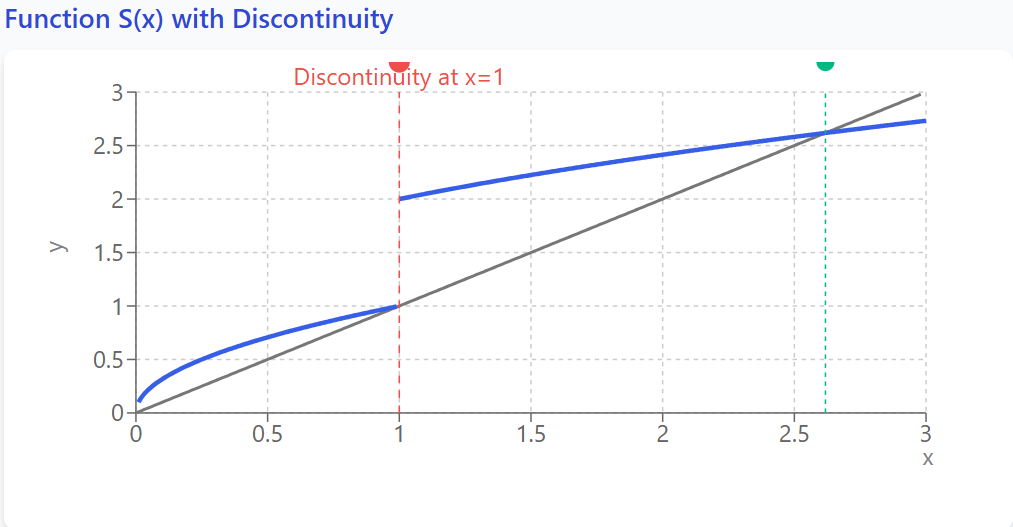
\includegraphics[width=1\linewidth]{Dynamic Programming/DP2/Chapter 1/Section 1.2/figure/discontinuous.png}
\end{figure}
    
\end{frame}

\begin{frame}{Convergence}
\begin{figure}
    \centering
    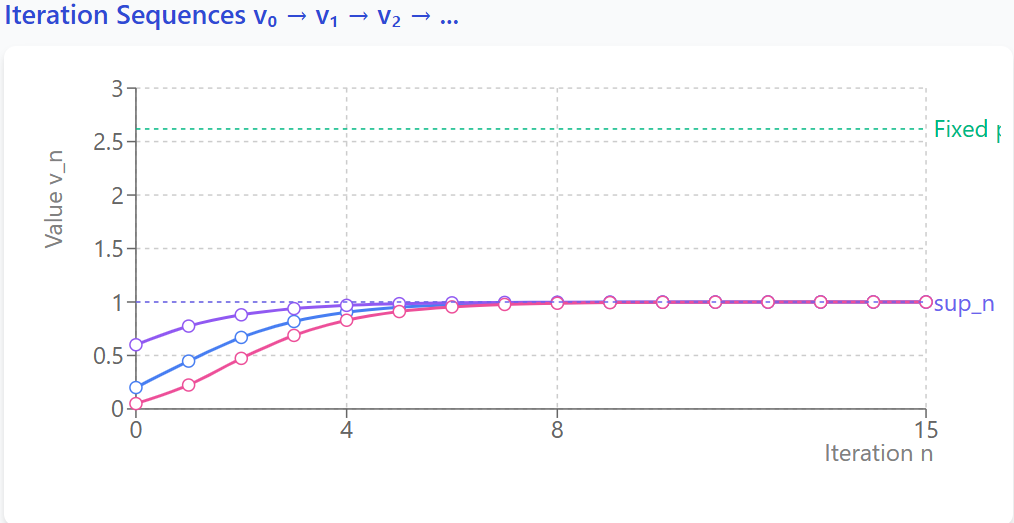
\includegraphics[width=1\linewidth]{Dynamic Programming/DP2/Chapter 1/Section 1.2/figure/convergence.png}
\end{figure}
\end{frame}

\begin{frame}{Order Completeness}
\begin{definition}
    A nonempty poset $V$ is called
    \begin{itemize}
        \item a \textbf{lattice} if every finite subset of $V$ has both a supremum and an infimum in $V$
        \item a \textbf{complete lattice} if every subset of $V$ has a supremum and an infimum in $V$
        \item \textbf{chain complete} if every chain in $V$ has a supremum and an infimum in $V$
        \item \textbf{$\sigma$-chain complete} is every at most countable chain in $V$ has a supremum and an infimum in $V$
    \end{itemize}
\end{definition}
\textbf{Remark:} Here  `finite' means nonempty finite, `at most countable' means empty, finite, or countable. 
    
\end{frame}

\begin{frame}{Chain complete poset is order bounded}

\begin{lemma}
    Let $V$ be any poset. We have
    \begin{itemize}
        \item $b:= \bigvee \emptyset$ exists in $V$ if and only if $V$ has a least element and that least element is $b$
        \item $u:= \bigwedge \emptyset$ exists in $V$ is and only if $V$ has a greatest element and that greatest element is $u$.
    \end{itemize}
\end{lemma}
    \begin{proof}
        Suppose $b=\bigvee\emptyset$ exists in $V$. By definition of empty set, we know that every subset of $V$ is an upper bound of $\emptyset$. In other words, every element of $V$ is in the upper bound of $\emptyset$. Hence, the least upper bound of the emptyset is the least element of $V$.\\
        \\
        Suppose $V$ has a least element and that least element is $b$. Following the above logic, the least upper bound of the emptyset should be the least element of $V$. Given its existence, we know that $b=\bigvee\emptyset$.
    \end{proof}
\end{frame}

\begin{frame}{Chain complete poset is order bounded}
\begin{lemma}
    d
\end{lemma}
    
\end{frame}



\end{document}
